%%%%%%%%%%%%%%%%%%%%%%%%%%%%%%%%%%%%%%%%%
% Jacobs Portrait Poster
% LaTeX Template
% Version 1.0 (31/08/2015)
% (Based on Version 1.0 (29/03/13) of the landscape template
%
% Created by:
% Computational Physics and Biophysics Group, Jacobs University
% https://teamwork.jacobs-university.de:8443/confluence/display/CoPandBiG/LaTeX+Poster
%
% Further modified by:
% Nathaniel Johnston (nathaniel@njohnston.ca)
%
% Portrait version by:
% John Hammersley
%
% The landscape version of this template was downloaded from:
% http://www.LaTeXTemplates.com
%
% License:
% CC BY-NC-SA 3.0 (http://creativecommons.org/licenses/by-nc-sa/3.0/)
%
%%%%%%%%%%%%%%%%%%%%%%%%%%%%%%%%%%%%%%%%%

%----------------------------------------------------------------------------------------
%	PACKAGES AND OTHER DOCUMENT CONFIGURATIONS
%----------------------------------------------------------------------------------------

\documentclass[final]{beamer}

\usepackage[scale=1.24]{beamerposter} % Use the beamerposter package for laying out the poster

\usetheme{confposter} % Use the confposter theme supplied with this template

\setbeamercolor{block title}{fg=ngreen,bg=white} % Colors of the block titles
\setbeamercolor{block body}{fg=black,bg=white} % Colors of the body of blocks
\setbeamercolor{block alerted title}{fg=white,bg=dblue!70} % Colors of the highlighted block titles
\setbeamercolor{block alerted body}{fg=black,bg=dblue!10} % Colors of the body of highlighted blocks
% Many more colors are available for use in beamerthemeconfposter.sty

%-----------------------------------------------------------
% Define the column widths and overall poster size
% To set effective sepwid, onecolwid and twocolwid values, first choose how many columns you want and how much separation you want between columns
% In this template, the separation width chosen is 0.024 of the paper width and a 4-column layout
% onecolwid should therefore be (1-(# of columns+1)*sepwid)/# of columns e.g. (1-(4+1)*0.024)/4 = 0.22
% Set twocolwid to be (2*onecolwid)+sepwid = 0.464
% Set threecolwid to be (3*onecolwid)+2*sepwid = 0.708

\newlength{\sepwid}
\newlength{\onecolwid}
\newlength{\twocolwid}
\newlength{\threecolwid}
\setlength{\paperwidth}{36in} % A0 width: 46.8in
\setlength{\paperheight}{48in} % A0 height: 33.1in
\setlength{\sepwid}{0.024\paperwidth} % Separation width (white space) between columns
\setlength{\onecolwid}{0.3\paperwidth} % Width of one column
%\setlength{\twocolwid}{0.464\paperwidth} % Width of two columns
\setlength{\threecolwid}{0.708\paperwidth} % Width of three columns
\setlength{\topmargin}{-0.5in} % Reduce the top margin size
%-----------------------------------------------------------

\usepackage{graphicx}  % Required for including images
\graphicspath{{../../images/}}

\usepackage{booktabs} % Top and bottom rules for tables

\usepackage{minted}

\usepackage{biblatex}
\bibliography{../../biblio.bib}

\usepackage{../../custom}

%----------------------------------------------------------------------------------------
%	TITLE SECTION
%----------------------------------------------------------------------------------------

\title{Sum-of-Squares Programming in Julia with JuMP} % Poster title

\author{Beno\^it Legat$^*$, Chris Coey$^\dagger$, Robin Deits$^\dagger$, Joey Huchette$^\dagger$ and Amelia Perry$^\dagger$}

\institute{$^*$ UCLouvain, $^\dagger$ MIT} % Institution(s)

%----------------------------------------------------------------------------------------

% https://tex.stackexchange.com/questions/426088/texlive-pretest-2018-beamer-and-subfig-collide
\makeatletter
\let\@@magyar@captionfix\relax
\makeatother

\begin{document}

\addtobeamertemplate{block end}{}{\vspace*{2ex}} % White space under blocks
\addtobeamertemplate{block alerted end}{}{\vspace*{2ex}} % White space under highlighted (alert) blocks

\setlength{\belowcaptionskip}{2ex} % White space under figures
\setlength\belowdisplayshortskip{2ex} % White space under equations

\begin{frame}[t,fragile] % The whole poster is enclosed in one beamer frame

\begin{columns}[t] % The whole poster consists of three major columns, the second of which is split into two columns twice - the [t] option aligns each column's content to the top

\begin{column}{\sepwid}\end{column} % Empty spacer column

\begin{column}{\onecolwid} % The first column
  \begin{block}{Sum-of-Squares (SOS) Programming}
  \begin{alertblock}{Nonnegative quadratic forms into sum of squares}
    \begin{center}
      \begin{tikzpicture}[scale=3]
        \draw[->, line width=2pt, bend left=30] (-1, 1.8) node[left] {$(x_1, x_2, x_3)$} to (-.1, 1.5);
        \draw[->, line width=2pt, bend left=30] (-1, 1.8) to (.9, 1.45);
        \draw[->, line width=2pt, bend right=30] (2.1, 2.2) node[right] {\alert{unique}} to (1.55, 1.55);
        \node at (-.2, 1.3) {$p(x)$};
        \node at (0.5, 1.3) {$=$};
        \node at (1.3, 1.3) {$x^\Tr Q x$};

        \node at (-1.9,  0.0) {$x_1^2 + 2x_1x_2 + 5x_2^2+ 4x_2x_3 + x_3^2$};
        %\node at (-1.4, -.3) {$+ 4x_2x_3 + x_3^2$};
        \node at (1.0, 0) {$=$};
        \node at (2.2, 0) {$x^\Tr \begin{pmatrix}1 & 1 & 0\\1 & 5 & 2\\ 0 & 2 & 1\end{pmatrix} x$};

        \node at (-2., -1.5) {$p(x) \geq 0$ $\forall x$};
        \node at (0.8, -1.5) {$Q \succeq 0$};
        \node at (-.3, -1.5) {$\Longleftrightarrow$};
        \draw[->, line width=2pt] (2.2, -1) to node[right] {cholesky} (2.2, -2.5);

        \node at (-2.6, -3.5) {$(x_1 + x_2)^2 + (2x_2 + x_3)^2$};
        %\node at (-2, -3.8) {$(2x_2 + x_3)^2$};
        \draw[->, line width=2pt] (.3, -3.5) to (-.3, -3.5);
        \node at (2.1, -3.5) {$x^\Tr \begin{pmatrix}1 & 1 & 0\\0 & 2 & 1\end{pmatrix}^\Tr \begin{pmatrix}1 & 1 & 0\\0 & 2 & 1\end{pmatrix} x$};
      \end{tikzpicture}
  \end{center}
  \end{alertblock}
  \begin{alertblock}{Nonnegative polynomial into sum of squares}
    \begin{center}
      \begin{tikzpicture}[scale=3]
        \draw[->, line width=2pt, bend left=30] (-1, 1.8) node[left] {$(x_1, x_2, x_3)$} to (-.1, 1.5);
        \draw[->, line width=2pt, bend left=20] (.6, 1.8) node[above] {$(x_1, x_1x_2, x_2)$} to (.9, 1.55);
        \draw[->, line width=2pt, bend right=30] (2.1, 2.2) node[right] {\alert{\emph{not} unique}} to (1.55, 1.55);
        \node at (-.1, 1.3) {$p(x)$};
        \node at (.5, 1.3) {$=$};
        \node at (1.3, 1.3) {$X^\Tr Q X$};
        \node at (-1.5, .3) {$x_1^2 + 2x_1^2x_2 + 5x_1^2x_2^2$};
        \node at (-1., -.3) {$+ 4x_1x_2^2 + x_2^2$};
        \node at (.5, 0) {$=$};
        \node at (1.8, 0) {$X^\Tr \begin{pmatrix}1 & 1 & 0\\1 & 5 & 2\\ 0 & 2 & 1\end{pmatrix} X$};

        \node at (-1.5, -1.5) {$p(x) \geq 0$ $\forall x$};
        \node at (1., -1.5) {$Q \succeq 0$};
        \node at (0., -1.5) {$\Longleftarrow$};
        \draw[->, line width=2pt] (2., -1) to node[right] {cholesky} (2., -2.5);

        \node at (-1.8, -3.2) {$(x_1 + x_1x_2)^2 +$};
        \node at (-1.8, -3.8) {$(2x_1x_2 + x_2)^2$};
        \draw[->, line width=2pt] (.2, -3.5) to (-.5, -3.5);
        \node at (2.1, -3.5) {$X^\Tr \begin{pmatrix}1 & 1 & 0\\0 & 2 & 1\end{pmatrix}^\Tr \begin{pmatrix}1 & 1 & 0\\0 & 2 & 1\end{pmatrix} X$};
      \end{tikzpicture}
    \end{center}
  \end{alertblock}

  \textbf{When is nonnegativity equivalent to sum of squares ?}

  Determining whether a polynomial is nonnegative is \alert{NP-hard}.

    \begin{description}
      \item[Hilbert 1888]
        Nonnegativity of $p(x)$ of $n$ variables and degree $2d$ is equivalent to sum of squares in the following three cases:
        \begin{itemize}
          \item $n = 1$ : Univariate polynomials
          \item $2d = 2$ : Quadratic polynomials
          \item $n = 2$, $2d = 4$ : Bivariate quartics
        \end{itemize}

      \item[Motzkin 1967]
        First explicit example:
        \[ x_1^4x_2^2 + x_1^2x_2^4 + 1 - 3x_1^2x_2^2 \geq 0 \quad \forall x \]
        but is \alert{not} a sum of squares.
        \begin{center}
          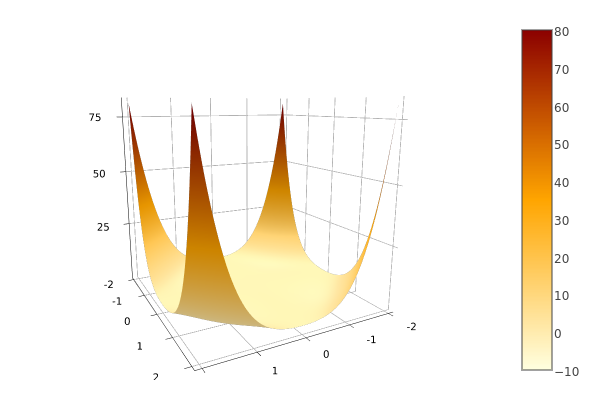
\includegraphics[trim=3cm .7cm 6cm 3cm, clip, width=0.7\textwidth]{motzkin.png}
        \end{center}
    \end{description}

  \end{block}

\end{column}

\begin{column}{\sepwid}\end{column} % Empty spacer column

\begin{column}{\onecolwid} % The second column
  \begin{block}{Manipulating Polynomials}
    Two implementations:
    %\begin{itemize}
      %\item
        \jlpkg{TypedPolynomials} and
      %\item
        \jlpkg{DynamicPolynomials}.
    %\end{itemize}

    One common independent interface: \jlpkg{MultivariatePolynomials}.
\begin{minted}{Julia}
@polyvar y # one variable
@polyvar x[1:2] # tuple/vector
\end{minted}
%    Build a polynomial from scratch:
%\begin{minted}{Julia}
%motzkin = x^4*y^2 + x^2*y^4 +
%          1 - 3x^2*y^2
%\end{minted}
    Build a vector of monomials:

    \begin{itemize}
      \item
        $(x_1^2, x_1x_2, x_2^2)$:
\begin{minted}{Julia}
X = monomials(x, 2)
\end{minted}
      \item
        $(x_1^2, x_1x_2, x_2^2, x_1, x_2, 1)$:
\begin{minted}{Julia}
X = monomials(x, 0:2)
\end{minted}
    \end{itemize}
  \end{block}

  \begin{block}{Polynomial variables}
    By hand, with an integer decision variable \texttt{a} and real decision variable \texttt{b}:
\begin{minted}{Julia}
@variable(model, a, Int)
@variable(model, b)
p = a*x^2 + (a+b)*y^2*x + b*y^3
\end{minted}
    From a polynomial basis, e.g. the
    \emph{scaled monomial} basis,
    with integer decision variables as coefficients:
\begin{minted}{Julia}
@variable(model,
          Poly(ScaledMonomialBasis(X)),
          Int)
\end{minted}
  \end{block}

  \begin{block}{Polynomial constraints}
    Constrain $p(x, y) \geq q(x, y)$ $\forall x, y$ such that $x \ge 0, y \ge 0, x + y \ge 1$ using the scaled monomial basis:
\begin{minted}{Julia}
S = @set x >= 0 && y >= 0 && x + y >= 1
@constraint(model, p >= q, domain = S,
            basis = ScaledMonomialBasis)
\end{minted}
    Interpreted as:
\begin{minted}{Julia}
@constraint(model, p - q in SOSCone(),
            domain = S,
            basis = ScaledMonomialBasis)
\end{minted}
    To use DSOS or SDSOS (Ahmadi, Majumdar 2017): %\cite{ahmadi2017dsos}:
\begin{minted}{Julia}
@constraint(model, p - q in DSOSCone())
@constraint(model, p - q in SDSOSCone())
\end{minted}
  \begin{alertblock}{SOS on algebraic domain}
    The domain $S$ is defined by equalities forming an \emph{algebraic variety}
    $V$ and inequalities $q_i$.
    We search for Sum-of-Squares polynomials $s_i$ such that
    \[ p(x) - q(x) \equiv s_0(x) + s_1(x) q_1(x) + \cdots \pmod{V} \]
    The Gr\"obner basis of $V$ is computed the equation is reduced modulo $V$.
  \end{alertblock}
  \end{block}

  \begin{block}{Dual value}
    The dual of the constraint is a positive semidefinite (PSD) matrix of moments $\mu$.
    The \texttt{extractatoms} function attempts to find an \emph{atomic} measure
    with these moments by solving an algebraic system.
  \end{block}
\end{column}

\begin{column}{\sepwid}\end{column} % Empty spacer column

\begin{column}{\onecolwid} % The third column
  \begin{block}{Sum-of-Squares extension}

    \begin{alertblock}{\jlpkg{MathOptInterface} (MOI)}
      MOI is an abstraction layer for mathematical optimization solvers.
      A constraint is defined by a ``function'' $\in$ ``set'' pair.
      %A few default sets are defined by it is \emph{extensible}.
    \end{alertblock}

    MOI extension:
    %\begin{itemize}
      %\item
        \texttt{AbstractVectorFunction} $\in$ \texttt{SOS(X)} (resp. \texttt{WSOS(X)}):
        SOS constraint without (resp. with) \texttt{domain}
        equipped with a bridge to \texttt{AbstractVectorFunction} $\in$ \texttt{PSD} (resp. \texttt{SOS(X)}).
    %\end{itemize}

    \begin{alertblock}{\JuMP{}}
      \JuMP{} is a domain-specific modeling language for mathematical optimization.
      It stores the problem directly (a cache can optionally be used) in the solver
      using MOI. % It is extensible by design.
    \end{alertblock}

    \JuMP{} extension:
    %\begin{itemize}
      %\item
        $p(x) \ge q(x)$ and $p(x) \in {}$\texttt{SOS()} are rewritten into
        MOI SOS or WSOS constraints, e.g.
        $x^2 + y^2 \ge 2xy$ is rewritten into
        $[1, -2, 1] \in {}$SOS$(x^2, xy, y^2)$.
        $p(x) \in {}$\texttt{DSOS()} (resp. \texttt{SDSOS()}) is rewritten into
        linear (resp. second-order cone) constraints.
    %\end{itemize}
  %\end{alertblock}


  %\vspace{10em}
  \begin{center}
  \begin{tikzpicture}[scale=3]
    \draw[rounded corners=20pt, fill=frambo!50] (-2, 1.5) rectangle (2, 2.5);
    \node at (0, 2) {\jlpkg{SumOfSquares}};
    \node at (0, 0) {
\includegraphics{JuMP.png}};
    \draw[->, line width=1mm] (0, 1.5) to (0, 0.3);
    \draw[rounded corners=20pt] (-3, -6.5) rectangle (3, -1.5);
    \node[rotate=90] at (-2.7, -4) {\jlpkg{MathOptInterface}};
    \node[rotate=-90] at (2.7, -4) {MOI};
    \draw[rounded corners=20pt, fill=lichen!70] (-1, -2.5) rectangle (1, -3.5);
    \node at (0, -3) {Bridging};
    \draw[->, line width=1mm] (0, -.8) to (0, -2.5);
    \draw[rounded corners=20pt, fill=aurore!70] (-1, -4.5) rectangle (1, -5.5);
    \node at (0, -5) {Caching};
    \draw[->, line width=1mm] (0, -3.5) to (0, -4.5);
    \draw[->, line width=1mm] (0, -5.5) to (-2, -7.5);
    \draw[->, line width=1mm] (0, -5.5) to (-1, -7.5);
    \draw[->, line width=1mm] (0, -5.5) to ( 0, -7.5);
    \draw[->, line width=1mm] (0, -5.5) to ( 1, -7.5);
    \draw[->, line width=1mm] (0, -5.5) to ( 2, -7.5);
    \draw[rounded corners=20pt, fill=canard!60] (-3, -8.5) rectangle (3, -7.5);
    \node at (0, -8) {Solvers: Mosek, CSDP, SCS...};
  \end{tikzpicture}
  \end{center}
  \begin{description}
    \item[\textbf{\textcolor{jblue!85}{Bridging}}] Automatic reformulation of a constraint into an equivalent
      form supported by the solver, e.g. quadratic constraint into second-order
      cone constraint. In particular, reformulates SOS/WSOS constraints
      into PSD constraints. An interior-point solver that natively supports
      SOS and WSOS % (SOS with \texttt{domain})
      without reformulation to SDP using
      the approach of (Papp, Y{\i}ld{\i}z 2017) % \cite{papp2017sum}
      is under development.
    \item[\textbf{\textcolor{jblue!85}{Caching}}] Cache of the problem data in case the solver do not support
      a modification (can be disabled). For instance, Mosek provides many
      modification capabilities in the API but CSDP only support
      pre-allocating and then loading the whole problem at once.
  \end{description}

  \end{block}

  %\begin{block}{References}
  %  \printbibliography
  %\end{block}

\end{column}

\end{columns} % End of all the columns in the poster

\end{frame}

\end{document}
